\section{Анализ Monte Carlo}

\subsection*{Генерация и отбор событий.}

Для отбора наилучших кандидатов было предложено использовать события, сгенерированные с помощью MC для распада $e^+e^- \to c\bar{c}$. На основе полученной статистики предлагается обучить модель Random Forest для отбора истинных событий на тагирующей стороне. Поскольку основной целью данной работы является измерение формфактора $\Lambda_c$, модель не будет использоваться для идентификации кандидатов на $\Lambda_c$ в исследуемой стороне.

Применяя аналогичные критерии отбора к тагирующей стороне, был добавлен канал $\Lambda_c^{\text{tag}} \to p K \pi$, что позволило увеличить статистическую значимость, исключив при этом канал $\Lambda_c \to \Lambda \ell \nu_\ell$ из анализа тагирующей стороны. В результате этого отбора удалось выделить следующее количество событий.

\begin{figure}[H]
    \centering
    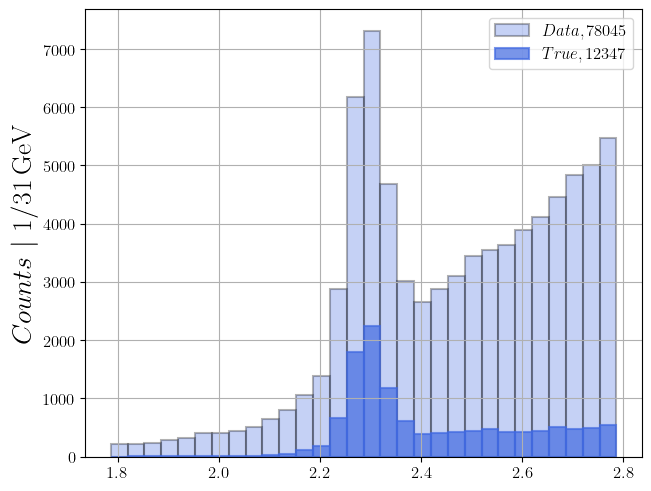
\includegraphics[width=0.7\linewidth]{img/mc_tr.png}
    \caption{Сгенерированные и отобранные события в MC, распределение по восстановленной массе $\Lambda_c$.}
\end{figure}


\subsection{Отбор истинных кандидатов в событиях Monte Carlo}


В качестве признаков использовались: $M^{rec}_{\Lambda_c}, \abs{p_{ach}}, M_{ach}, \abs{p_{\pi}}, M_{\pi}, \abs{p_{X_c}}, \abs{p_{X_c}}, M_{X_c}, E_{cm}, \abs{p_{cm}}$, и углы между ними и главное предполагаемый канал распада $X_c$, были введены следующие обозначения $ach$ --- носистель $\bar c$,  $cm$ --- система центра масс. Целевая метка определялась из информации присвоенным MC генератором.


Для обучения был использован Random Forest классификатор с количеством деревьев 4000, глубиной деревьев до 200 и настройкой параметров для борьбы с несбалансированностью классов. Модель обучалась на 60\% данных, оставшиеся 40\% использовались для тестировани.


Для оценки производительности модели был построен ROC-кривая и рассчитана площадь под кривой (AUC). Кроме того, предсказанные вероятности были использованы для выбора порога вероятности, выше которого событие классифицируется как содержащее истинного кандидат

\begin{figure}[H]
    \centering
    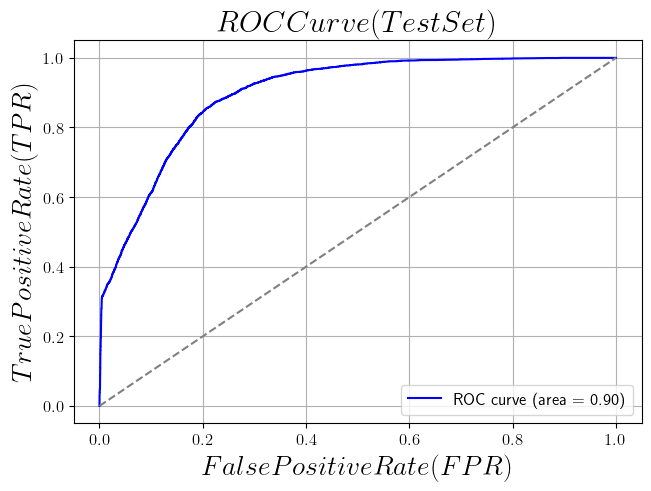
\includegraphics[width=0.7\linewidth]{img/ROC_f.png}
    \caption{ROC кривая первого классификатора.}
\end{figure}


Поскольку в одном событии может быть несколько комбинаций, на каждом шаге выполнялась фильтрация кандидатов. Сначала отбирались события с вероятностью больше порога $L = 0.4$, а затем среди всех кандидатов в одном событии выбирался лучший на основе максимальной вероятност


Были построены гистограммы для сравнения истинных и предсказанных кандидатов, а также для анализа ошибок классификации (FP, FN, TP, TN). Это позволило оценить распределение признаков для разных категорий событий и уточнить работу классификатора на тестовой выборке.

\begin{figure}[H]
    \centering
    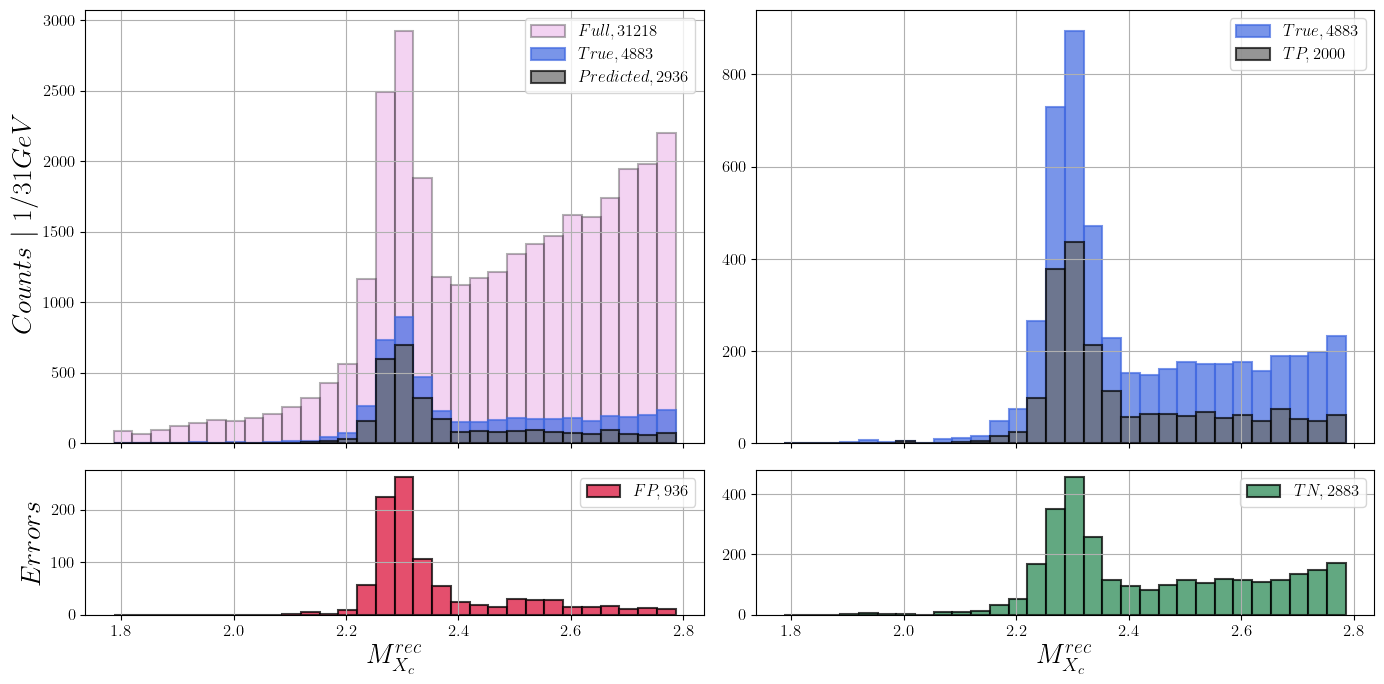
\includegraphics[width=1\linewidth]{img/MC_res.png}
    \caption{Результаты второго классификатора на тестовой выборке.}
\end{figure}
